\chapter{Eigener Ansatz}

\section{Zielsetzung}
Die vorliegende Arbeit handelt davon mit Hilfe eines eigens erstellten 3D Modells eine Drohne Indoor navigieren zu können. Um dies umsetzen zu können gibt es einen Quadrokopter der zu diesem Zwecke eingesetzt werden kann. \\
Heutzutage basiert die Navgiation vieler Drohnen auf \ac{GPS} allerdings kann man Drohnen innerhalb von Gebäuden nicht mit dieser Technik fliegen lassen, da damit die im Innenraum vorhandenen Hindernisse nicht berücksichtigt werden können. Aus diesem Grund soll hierfür eine Möglichkeit gefunden werden, welche es ermöglicht eine Drohne ohne \ac{GPS} im Innenraum eines Gebäudes mit Hilfe eines 3D Modells navigeren zu können.\\
Der Quadrokopter, die Coex Clover Drohne ist bereits mit verschiedenen Sensoren ausgestattet und kann potientiell mit weiteren Sensoren erweitert werden. Jedoch ist die Drohne bis zum Beginn dieser Arbeit noch nicht richtig geflogen ist. Somit muss zum einen die Nutzbarkeit der Drohne für dieses Projekt sichergestellt werden, um diese in dieser Arbeit einsetzen zu können. \\
Ziel dieser Arbeit ist es, bestenfalls den bereits vorhandenen Quadrokopter mit Hilfe eines eigens erstellten 3D Umweltmodells innerhalb eines Raumes navigieren zu können und dadurch kleinere Aufgaben wie beispielsweise das Auslesen eines QR-Codes somit erledigen zu können.



\section{Vorgehensweise}

In Abbildung \ref{fig:vorgehensweise} sind die 2 Vorgehensweisen die wir uns ausgedacht haben ersichtlich. In Ansatz 1 hatten wir zuerst versucht ein vorher gescanntes 3D Modell auf die Drohne zu laden und eine Positionierung im 3D Modell durchzuführen. Schnell wurde ersichtlich das es wenig sinnvoll eine Positionierung in einem vorher bekannten 3D Modell durchzuführen, da die Dronhe auch in unbekannten Umgebungen eingesetzt werden soll. Deshalb ist es sinnvoller die Positionierung und die 3D Modell Erstellung zu kombinieren. Dazu kann \ac{SLAM} eingesetzt werden. Deshalb haben wir Ansatz 1 relativ schnell wieder verworfen.

\begin{figure}
    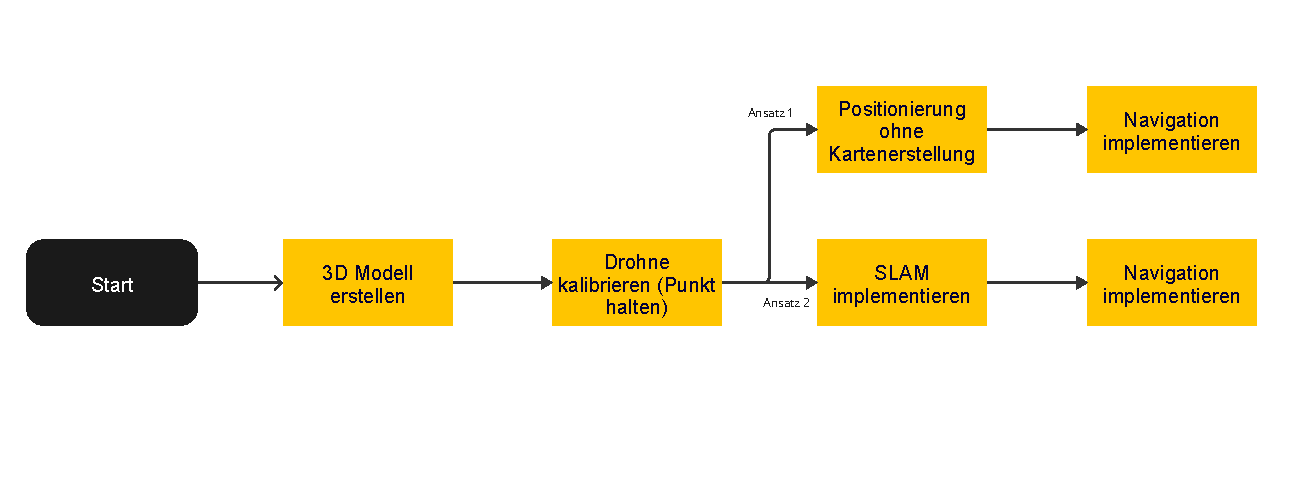
\includegraphics[scale=0.7]{images/ansatz_plan.pdf}
    \caption{Geplante Vorgehensweise}\label{fig:vorgehensweise}
\end{figure}

\subsection{Auswahl SLAM Algorithmus}

Mehrere \ac{SLAM} Algorithmen standen zur Auswahl, aufgrund der limitierten Performance des Raspberry PIs, haben wir den Algorithmus mit den kleinsten Anforderungen gewählt.

\subsubsection{OBD-SLAM3}

BD-SLAM3 ist eine Erweiterung des OBD-SLAM (Oriented Bounding Box SLAM) Algorithmus, der für die simultane Lokalisierung und Kartierung (SLAM) in dreidimensionalen Umgebungen entwickelt wurde. Im Gegensatz zu OBD-SLAM verwendet OBD-SLAM3 jedoch eine tiefere Netzwerkarchitektur, um die Leistung und Genauigkeit der Odometrie und der visuellen Wahrnehmung zu verbessern.

OBD-SLAM3 nutzt eine Kombination aus Tiefenkameras und RGB-Kameras, um eine 3D-Repräsentation der Umgebung zu erstellen und gleichzeitig die Bewegung des Roboters in der Umgebung zu schätzen. Der Algorithmus verwendet ein neuronales Netzwerk, um die Tiefeninformationen der Kameras zu verarbeiten und eine Schätzung der Kamerapositionen und -orientierungen zu generieren.

Im Gegensatz zu anderen SLAM-Verfahren, die auf einer Vielzahl von Features wie Punkten oder Linien basieren, nutzt OBD-SLAM3 Oriented Bounding Boxen (OBBs), um eine robustere Schätzung der Kamerabewegungen und -positionen zu ermöglichen. Die OBBs erlauben eine genauere Modellierung der Umgebung und eine bessere Korrektur von Fehlern, die durch Ungenauigkeiten bei der Berechnung von 3D-Points entstehen können.

Insgesamt ermöglicht OBD-SLAM3 eine genauere und robustere Lokalisierung und Kartierung in dreidimensionalen Umgebungen, was ihn zu einem vielversprechenden Ansatz für autonome Robotikanwendungen macht.

\subsubsection{LSD-SLAM}

LSD-SLAM (Large-Scale Direct Monocular SLAM) ist ein Algorithmus zur simultanen Lokalisierung und Kartierung (SLAM) in Echtzeit, der eine einzelne Kamera verwendet. Im Gegensatz zu anderen SLAM-Methoden, die Merkmale oder Punktwolken verwenden, um eine Karte der Umgebung zu erstellen, nutzt LSD-SLAM eine direkt auf den Bildern basierende Methode. Hierbei werden die Intensitäts- und Gradienteninformationen der Bilder genutzt, um die Kameraposition und -orientierung zu schätzen und eine dichte Punktwolke der Umgebung zu erstellen.

LSD-SLAM wurde von Jakob Engel, Thomas Schöps und Daniel Cremers an der Technischen Universität München entwickelt und im Jahr 2014 vorgestellt. Es hat sich als eine effektive Methode zur SLAM-Problemstellung erwiesen, insbesondere in Umgebungen mit geringer Textur oder schlechter Beleuchtung.



\subsection{Auswahl Lokalisierungssystem}

Die in Kapitel \ref{lst:navigation-types} vorgestellten Vorgehensweisen sind mehr oder weniger geeignet für den Einsatz auf der Drohne und für dein Einsatz mit \ac{SLAM}
In einer gewichteten Analyse wurden die einzelnen Vorgehensweisen verglichen und der Gewinner ausgewählt.

Verglichen wurden Navigationstypen nach den in Tabelle \ref{tab:vergleich-kriterien} genannten Kiterien.

Die Kriterien werden in Tabelle \ref{tab:vergleich} gegenübergestellt und in Tabelle \ref{tab:vergleich-gewichtung} werden Sie gewichtet.

Die Einschätzungen für die Gewichtungen in der Tabelle basieren auf der subjektiven Einschätzung der Bedeutung jedes Kriteriums für das \ac{SLAM}-Navigationssystem. Die Gewichtungen können auf verschiedenen Faktoren basieren, darunter:

\begin{itemize}
\item \textbf{Anforderungen des Projekts:} Die Gewichtungen können durch die spezifischen Anforderungen des Projekts bestimmt werden. Wenn beispielsweise eine besonders hohe Genauigkeit erforderlich ist, kann diesem Kriterium eine höhere Gewichtung zugeordnet werden.

\item \textbf{Wichtigkeit für den Einsatzzweck:} Die Gewichtungen können auf der Wichtigkeit jedes Kriteriums für den vorgesehenen Einsatzzweck des SLAM-Navigationssystems basieren. Wenn beispielsweise das System in einer Umgebung mit vielen Störungen eingesetzt wird, kann der Anfälligkeit für Störungen eine höhere Gewichtung zugeordnet werden.
\item \textbf{Expertenmeinungen} Expertenmeinungen: Die Gewichtungen können auf Expertenmeinungen basieren, die auf ihrer Erfahrung und Fachkenntnis in der Navigationstechnologie beruhen.
\end{itemize}

Aufgrund des Ergebnisses aus Tabelle \ref{tab:vergleich-gewichtung} wird ersichtlich das folgende Lokalisierungsvorgehensweisen für den Einsatz mit der Drohne und SLAM am besten eingesetzt werden können.

\begin{itemize}
    \item Optical Sensoren
    \item Inertial Navigation
\end{itemize}

Aufgrund der Tatsache, dass die zur Verfügung stehende COEX Drohne bereits auch über Inertial Sensoren verfügt, kann damit die Qualität von \ac{SLAM} noch weiter verbessert werden.

Alleine mit Inertial Navigation kann kein \ac{SLAM} durchgeführt werden. Da die Inertial Navigation keine Kenntniss der Umgebung hat. Dies ist alleine ebenso ein Punkt, der die alleinige Verwendung von Inertial Navigation verhindert.

\begin{table}[h]
    \centering
    \begin{tabular}{|p{5cm}|p{5cm}|p{5cm}|}
        \hline
        \textbf{Kriterien} & \textbf{Gewichtung} & \textbf{Begründung} \\
        \hline
        Genauigkeit & 5 & Um eine möglichst akkurate Hindernisserkennung zu ermöglichen, sollte das Lokalisierungssystem genau sein. \\
        \hline
        Ungenauigkeitsakkumulation & 5 & Wie stark summieren sich die Fehler auf? \\
        \hline
        Umgebungserfordernisse & 10 & Welche Anforderungen werden an die Umgebung gestellt? Müssen spezielle Eigenschaften der Umgebung beachtet werden? \\
        \hline
        Anfälligkeit für Störungen & 2 & Wie anfällig ist das System für Störungen? \\
        \hline
        Anwendungsbereiche & 20 & In welchen Anwendungsbereichen kann das System eingesetzt werden? \\
        \hline
    \end{tabular}
    \caption{Vergleichskriterien}
    \label{tab:vergleich-kriterien}
\end{table}
\begin{table}


\begin{center}
   \fontsize{7}{11}\selectfont
    \begin{tabular}{|p{2cm}|p{2cm}|p{2cm}|p{3cm}|p{2cm}|p{3cm}|}
    \hline
    \textbf{Lokalisier\-ungsart} & \textbf{Genauigkeit} & \textbf{Ungenauigkeits\-akkumulation} & \textbf{Umgebungs\-erfordernisse} & \textbf{Anfälligkeit für Störungen} & \textbf{Anwendungsbereiche} \\\hline
    Inertial Navigation & Mittel bis hoch & Ja & Keine spezifischen Anforderungen & Gering & Innen- und Außenbereiche, aber keine Erkennung der Umgebung \\\hline
    Optische Sensoren & Mittel bis hoch & Nein & Gut strukturierte Umgebung mit markanten Merkmalen & Mittel bis hoch & Innen- und Außenbereiche \\\hline
    Ultraschall- oder Infrarotsensoren & Niedrig bis mittel & Ja & Hindernisse müssen reflektierend sein & Mittel bis hoch & Innenbereiche \\\hline
    Magnetfeld\-sensoren & Niedrig bis mittel & Ja & Geringe Magnetfeldstörungen & Hoch & Innenbereiche ohne starke magnetische Störungen, aber keine Erkennung der Umgebung \\\hline
    Funkbasierte Lokalisierung & Niedrig bis mittel & Nein & Ausreichende Abdeckung mit Funkquellen & Gering & Innen- und Außenbereiche, aber keine Erkennung der Umgebung \\\hline
    \end{tabular}
    \caption{Vergleich Lokalisierungsmethoden}\label{tab:vergleich}
    \end{center}
\end{table}

\begin{table}[ht]
    \fontsize{6}{11}\selectfont
    \begin{center}
        \begin{tabular}{|p{2cm}|p{1.3cm}|p{2cm}|p{1.5cm}|p{2cm}|p{2cm}|p{1.5cm}|}
            \hline
            \textbf{Lokalisier\-ungsart} & \textbf{Genauig\-keit} & \textbf{Ungenauigkeits\-akkumulation 0=Ja 10=Nein} & \textbf{Umgebungs\-erfordernisse} & \textbf{Anfälligkeit für Störungen} & \textbf{Anwendungs\-bereiche} & \textbf{Summe der Punkte} \\\hline
            \rowcolor{green}
            Inertial Navigation & $8*5=40$ & $0*10=0$ & $10*10=100$ & $9*2=18$ & $10*20=200$ & 358 \\\hline
            \rowcolor{green}
            Optische Sensoren & $7*5=35$ & $10*10=100$ & $7*10=70$ & $3*2=6$ & $10*20=200$& 411 \\\hline
            Ultraschall- oder Infrarotsensoren & $4*5=20$ & $0*10=0$ & $3*10=30$ & $3*2=6$ & $10*20=200$& 256 \\\hline
            Magnetfeldsensoren & $2*5=10$ & $0*10=0$ & $2*10=20$ & $1*2=2$ & $7*20=140$ & 172 \\\hline
            Funkbasierte Lokalisierung & $1*5=5$ & $0*10=0$ & $0*10=0$ & $8*2=16$ & $10*20=200$ & 221 \\\hline
        \end{tabular}
        \caption{Gewichtete Analyse}\label{tab:vergleich-gewichtung}
    \end{center}
\end{table}

\subsection{Auswahl \ac{SLAM} Algorithmus}






